\documentclass[12pt]{article}
\usepackage[margin=1.0in]{geometry}
\usepackage{amsmath,amsthm,amssymb,amsfonts}
\usepackage{enumerate,mathtools}
\usepackage{pgfplots}
\usepackage{tikz,tkz-euclide}
\usepackage{siunitx}
\usepackage{pgfplots}
\usetikzlibrary{calc}
\usetikzlibrary{positioning}
\usetkzobj{all}
\usepackage{caption}
\usepackage{float}
\usepackage{scrextend}

\newtheorem{theorem}{Theorem}[section]
\graphicspath{ {./images/} }

\title{Constructing the Shortest Hamiltonian\\Path via Bijection Ranges}
\author{
Mark Wesley Harris
}
\date{\today}

\begin{document}
\maketitle

\section{Introduction}\label{sec:intro}
This document breifly explains the theoretical concepts behind the
Shortest Path Algorithm developed in the GitHub
pixarninja/shortest\_path\_algorithm repository. This algorithm attempts
to solve the Traveling Salesman Problem, with the input of a 2D graph of datapoints
represented on a Cartesian coordinate system.

\section{Definitions}\label{sec:def}
\begin{itemize}
\item $(x,y)$: the definition of a point with coordinates $(x,y)$.
\item $<p,q>$: the definition of a vector from point $p$ to point $q$.
\item $[s_1, s_2, ..., s_k]$: the definition for a path through a known set of edges.
\item $n$: the number of points in the dataset.
\item $\mathcal{V}$: the set of all vertices in the dataset.
Formally, $\mathcal{V} = \{p_1, p_2, ..., p_n\}$
\item $\mathcal{E}$: the set of all edges in the dataset.
The size of $\mathcal{E}$ is $n \times n$.
\item $\mathcal{H}$: the convex hull of the dataset.
Formally, $\mathcal{H} = \{h_1, h_2, ..., h_k\}$, where $k \leq n - 1$.
Given any set of points,
there is only one convex hull.
\item $\mathcal{S}$: the shortest path of a dataset as the set
$\mathcal{S} = \{s_1, s_2, ..., s_n\}$
of edges which are contained in the shortest path.
\item $\mathcal{E}'$: the set of all edges in the dataset that are in $\mathcal{E}$
but not $\mathcal{S}$.
Formally, $\mathcal{E}' = \mathcal{E} - \mathcal{S}$.
\item $\mathcal{W}$: the set of edges produced by the construction phase of the algorithm.
Formally, $\mathcal{W} = \{w_1, w_2, ..., w_m\}$, where $3 < m < n^2$.
\item $\mathcal{S}' \equiv \mathcal{S}$: the path $\mathcal{S}'$ has the same
perimeter as path $\mathcal{S}$
(they may or may not have the same edges).
\end{itemize}

\section{Theoretical Concepts}\label{sec:theory}
My algorithm is based upon many theoretical concepts I have discovered through
research and experimentation. They are explained below
Sections \ref{subsec:props} and \ref{subsec:invalid}.

\subsection{Properties of Shortest Paths}\label{subsec:props}
I begin by describing the properties I have found to be true for all shortest
paths. These properties have been used to create the foundations for my algorithm.
\begin{enumerate}
\item For any two edges $s_i,s_j \in \mathcal{S}$ where
$i \neq j$, $s_i$ and $s_j$ do not cross. 
\item For any two edges $s_i,s_j \in \mathcal{S}$ where
$i \neq j$, $s_i$ and $s_j$ do not overlap. 
\item No edge $s \in \mathcal{S}$ intersects a point
$p \in \mathcal{V}$ where $s_1,s_2 \neq p$.
I.e. if an edge $e$ intersects a point $p$ that isn't an end point of $e$,
then $e \notin \mathcal{S}$.
\item If we were to add an arbitrary point $p_{n+1}$ to $\mathcal{V}$,
the form of $\mathcal{S}$
will not change iff $p_{n+1}$ is a point on the line of any $s \in \mathcal{S}$.
Thus $\exists s \in \mathcal{S}$ such that $p_{n+1}$ lies on $s$.
\end{enumerate}

\subsection{Invalidating a Segment}\label{subsec:invalid}
My algorithm is based upon the concept of invalidating as many segments of $\mathcal{E}$
as possible, but keeping all segments which are probably in $\mathcal{S}$.
In order to do this,
I propose a method of edge construction that begins with a complete graph
and invalidates edges based upon the
properties for shortest paths which I have produced
above. Any segment which fails these properties is not likely in $\mathcal{S}$,
and so it should not be included in $\mathcal{W}$.

\section{Bijection Range Method}\label{subsec:bijection-range-method}
The properties discussed in Section \ref{subsec:props} are not easily enforced
on a given dataset. I have interpretted them as illustrated by the following guidelines:
\begin{enumerate}
\item We are given a generic segment $e \in \mathcal{E}$ with endpoints
$e_1,e_2 \in \mathcal{V}$.
\item Take any two points $p,q \in \mathcal{V}$ such that $p \neq e_1,e_2$
and $q \neq e_1,e_2$.
\item Take all points $x$ on the continuous line $e$ where
$x \notin \mathcal{V}$.
\item Test if the distance of $[p,x]$ plus the distance of $[q,x]$
is less than the distances of $[e_1,x]$ plus the distances of
$[p,x]$, $[q,x]$, or $[x,e_2]$. In other words,
test if the path from $p$ to $q$ through $x$
is shorter than any path from a point in the test set $\mathcal{T} = \{e_1, e_2, p, q\}$
to any other point in $\mathcal{T}$ through $x$.
\item If true, then $e \notin \mathcal{W}$.
Otherwise it is shown that $e$ statisfies the
properties in Section \ref{subsec:props}, so $e \in \mathcal{W}$.
\end{enumerate}
My goal is to enforce the rule that if a new point $p_{n + 1}$ was added
to $\mathcal{V}$ and it were to lie on
any edge $w \in \mathcal{W}$, the form of $\mathcal{S}$ would not change.
\\\\
It is obvious that checking all possible points for all possible segments presents
a challenge in time complexity. Even assuming that checking all points $x$ on segment
$e \in \mathcal{E}$ takes a polynomial amount of time --- let's say this value is some
polynomial $f(n) = a_np^n + a_{n - 1}p^{n - 1} \dots + a_1p + a_0$ ---
it would be multiplied by checking each edge against each other edge, which
without any simplification is $O(n^4)$. Thus even if the degree of function $f$ is
relatively low, running the solution on large datasets is infeasible in practice.
\\\\
The following subsections discuss possible solutions to this complexity
problem. What is implmented in the algorithm is the Bijection Range Abstraction Method,
defined in Section \ref{subsec:bijection-range-method}.

\subsection{Intersection Method}\label{subsec:intersection-method}
The Bijection Range Method works for determining ranges on a segment $e$
for which points $p,q \in \mathcal{V}$ are closer to $e$ than
the endpoints $e_1$ or $e_2$.
However, since we are only interested
in invalidating the line with respect to this property, it is worth looking at
the possibility of using the intersection of any $e' \in \mathcal{E}$
with $e$ instead.
\begin{theorem}\label{thm:overlap}
Given a line segment $e \in \mathcal{E}$ with endpoints $e_1,e_2 \in \mathcal{V}$,
for each $p,q \in \mathcal{V}$ where $p \neq e_1,e_2$ and $q \neq e_1,e_2$,
if $p$ and $q$ have overlapping Bijection Ranges and
form a convex quadralateral with their lower and upper bound intersection points,
then the segment $e'$ passing through $p$ and $q$ intersects $e$.
\end{theorem}
\begin{proof}
The proof is shown below:
\begin{enumerate}[(1)]
\item Given that $p$ and $q$ have overlapping Bijection Ranges,
it is evident that there are 2 intersection points formed by
the lower and upper bounds of the intersection of ranges.
Let these points be $l$ and $u$, respectively.
\item By definition, these points form a quadralateral.
As given, the qudralateral is convex. Thus the source point of a Bijection Range
will never extend passed a lower or upper bound.
Let the quadralateral $p,l,q,u$ be denoted as $Q$.
\item Since $Q$ is a convex quadralateral,
a line segment can be drawn between $p$ and $q$ that lies within
the inner region formed by $Q$.
Let that line be denoted as $e'$.
\item Since $l$ and $u$ both intersect $e$, and $e'$ is a continuous line
that lies between $l$ and $u$, then $e'$ must also intersect $e$.
\end{enumerate}
\end{proof}

The Intersection Method is a valid approach to determine if two Bijection Ranges
intersect, however the requirement that the two ranges form a convex quadralateral is
not a trivial calculation. Therefore another method was developed
to determine if two Bijection Ranges overlap. This method is called
Bijection Range Abstraction, and was used in the final implementation of the algorithm.

\subsection{Bijection Range Abstraction}\label{subsec:bijection-range-method}
Calculating both bijections of each possible point $v \in \mathcal{V}$
for each edge $e \in \mathcal{E}$
is a very costly method of validating a segment. Instead of having to do the calculations
each time, it would be nice if there were a mathematical area to represent
when a point's bijection ranges will overlap for a given segment.
\begin{theorem}\label{thm:semicircle}
The area in which there is a bijection range created from point $p \in \mathcal{V}$
using segment $w \in \mathcal{E}$
can be represented as a semicircle, $M$, where $w$ is the segment opposite its arc.
\end{theorem}
\begin{proof} The proof is shown below:
\begin{enumerate}[(1)]
\item Let $w$ be the edge we are testing, with points $w_1,w_2 \in \mathcal{V}$.
\item Take a point $p \in \mathcal{V}$ where $p \neq w_1,w_2$ and $p$ does not lie on $w$.
\item Let $M$ be the unique semicircle in the direction of $p$ formed using $w$ as the
flat segment of $M$.
\item Let $A$, $B$, and $C$ represent the points $w_1$, $p$, and $w_2$, respectively.
Similarly, let $D$, $E$, and $F$ represent the midpoints of segments
$AC$, $BC$, and $AC$, respectively.
\item Now we assume the 3 cases for the position of $p$ relative to $M$:
\begin{enumerate}[(i)]
\item Assume that $p$ lies on the arc of semicircle $M$:
\begin{figure}[h!]
\begin{center}
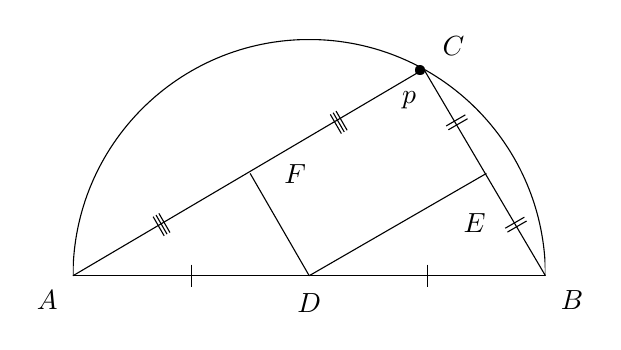
\begin{tikzpicture}
% A clipped circle is drawn
\begin{scope}
    \clip (-3,0) rectangle (3,3);
    \draw (0,0) circle(3);
    \draw (-3,0) -- (3,0);
\end{scope}
\coordinate (A) at (-3,0);
\coordinate (B) at (3,0);
\coordinate (C) at (60:3);
\coordinate (D) at (0,0);
\coordinate (E) at (2.25,1.29905);
\coordinate (F) at (-0.75,1.29905);
\tkzMarkSegment[color=black,pos=.5,mark=|](A,D)
\tkzMarkSegment[color=black,pos=.5,mark=|](D,B)
\tkzMarkSegment[color=black,pos=.5,mark=||](B,E)
\tkzMarkSegment[color=black,pos=.5,mark=||](E,C)
\tkzMarkSegment[color=black,pos=.5,mark=|||](A,F)
\tkzMarkSegment[color=black,pos=.5,mark=|||](F,C)
\draw (-3,0) -- (61:3); % AC
\draw (3,0) -- (61:3); % BC
\draw (0,0) -- (2.25,1.29905); % DE
\draw (0,0) -- (-0.75,1.29905); % DF
\node[right = -3mm of (60:3)] {\textbullet}; % p
%%Labels for the vertices are typeset.
\node[below left = 1mm of {(-3,0)}] {$A$};
\node[below right = 1mm of {(3,0)}] {$B$};
\node[above right = 1mm of {(60:3)}] {$C$};
\node[below = 2.5mm of {(65:3)}] {$p$};
\node[below = 1mm of {(0,0)}] {$D$};
\node[below left = 5mm of {(25:3)}] {$E$};
\node[below right = 15mm of {(120:3)}] {$F$};
\end{tikzpicture}
\end{center}
\caption{$p$ lies on $M$}\label{fig:case1}
\end{figure}
See Figure \ref{fig:case1} as a reference for the steps discussed below.
\begin{enumerate}[(a)]
\item Points $A$, $B$, and $C$ satsify the requirements of Thale's Theorem:
``if segment $AB$ is a diameter, then the angle at $C$ is a right angle.''
Thus $\angle ACB = 90$.
\item Let vector $V$ be the bijection of $BC$, so that $V$ passes through
$E$ and is perpendicular to $BC$.
Let the intersection point of $V$ and $AC$ be point $I$.
\item Since $\angle ABC$ = $\angle IBE$ and $\angle BCA = \angle BEI$,
$\triangle ABC$ and $\triangle IBE$ are similar triangles.
\item Given that $BE$ is half the length of $BC$,
then $BI = \frac{BA}{2} = BD$.
Thus $I$ is halfway between $A$ and $B$, so $I \equiv D$.
\item Now let $V$ be the bijection of $AC$, so that $V$ passes through
$F$ and is perpendicular to $AC$.
Let the intersection point of $V$ and $AC$ be point $I$.
\item Since $\angle BAC$ = $\angle IAF$ and $\angle ACB = \angle AFI$,
$\triangle ABC$ and $\triangle AIF$ are similar triangles.
\item Given that $AF$ is half the length of $AC$,
then $AI = \frac{BA}{2} = AD$.
Thus $I$ is halfway between $A$ and $B$, so $I \equiv D$.
\item Since both bijections for $p$ meet in the center of $w$,
the Bijection Range is a single point.
\end{enumerate}
This shows that the Bijection Range for points along the arc of $M$ are equal to
the center $w$.
\\\\
\item Now assume that $p$ lies inside the area of $M$ but not on the arc of $M$:
\begin{figure}[h!]
\begin{center}
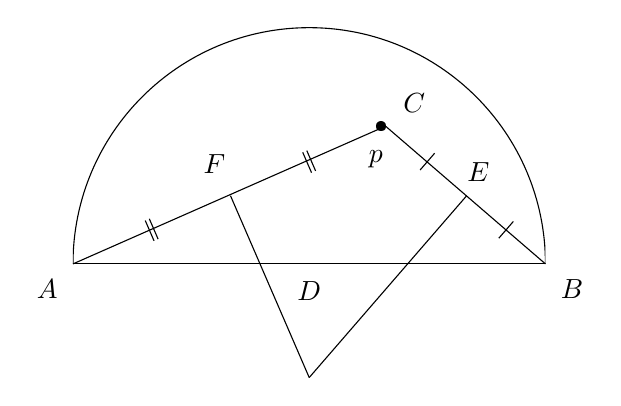
\begin{tikzpicture}
% A clipped circle is drawn
\begin{scope}
    \clip (-3,0) rectangle (3,3);
    \draw (0,0) circle(3);
    \draw (-3,0) -- (3,0);
\end{scope}
\coordinate (A) at (-3,0);
\coordinate (B) at (3,0);
\coordinate (C) at (60:2);
\coordinate (D) at (0,0);
\coordinate (E) at (2,0.86605);
\coordinate (F) at (-1,0.86605);
\tkzMarkSegment[color=black,pos=.5,mark=|](B,E)
\tkzMarkSegment[color=black,pos=.5,mark=|](E,C)
\tkzMarkSegment[color=black,pos=.5,mark=||](A,F)
\tkzMarkSegment[color=black,pos=.5,mark=||](F,C)
\draw (-3,0) -- (61:2); % AC
\draw (3,0) -- (61:2); % BC
\draw (0,-1.443352) -- (2,0.86605); % DE
\draw (0,-1.443352) -- (-1,0.86605); % DF
\node[right = -3mm of (60:2)] {\textbullet}; % p
%%Labels for the vertices are typeset.
\node[below left = 1mm of {(-3,0)}] {$A$};
\node[below right = 1mm of {(3,0)}] {$B$};
\node[above right = 1mm of {(60:2)}] {$C$};
\node[below = 2.5mm of {(65:2)}] {$p$};
\node[below = 1mm of {(0,0)}] {$D$};
\node[above right = 1mm of {(25:2)}] {$E$};
\node[below left = 6mm of {(105:2)}] {$F$};
\end{tikzpicture}
\end{center}
\caption{$p$ lies inside $M$}\label{fig:case2}
\end{figure}
See Figure \ref{fig:case2} as a reference for the steps discussed below.
\begin{enumerate}[(a)]
\item As shown above, if $p$ is on the arc of $M$ then $\angle ACB = 90$.
Thus if $p$ is inside the arc, $\angle ACB < 90$ or $\angle ACB > 90$.
\item As $p$ approaches $w$, $\angle ACB$ approaches $180$. So $\angle ACB > 90$.
\item Since $\angle ACB > 90$,
the two bijection vectors will intersect somewhere below $w$,
opposite to $M$.
\item The area between the intersections of these vectors with $w$ is
the Bijection Range found previously through iteration.
\end{enumerate}
This shows that the Bijection Range for points inside the area of $M$ is equal to the
intersection of the bijection vectors with $w$.
\\\\
\item Now assume the final case, that $p$ lies outside the area of $M$ but not on
the arc of $M$:
\begin{figure}[h!]
\begin{center}
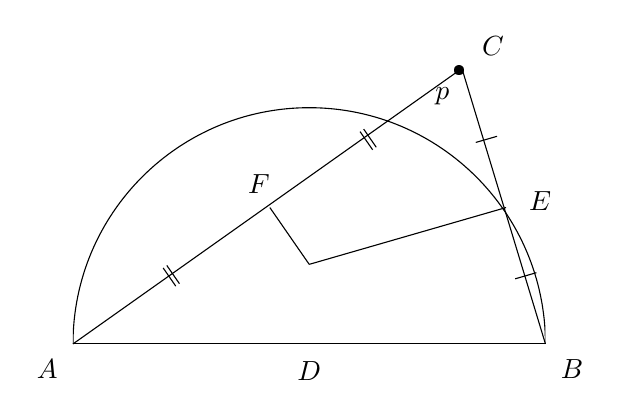
\begin{tikzpicture}
% A clipped circle is drawn
\begin{scope}
    \clip (-3,0) rectangle (3,3);
    \draw (0,0) circle(3);
    \draw (-3,0) -- (3,0);
\end{scope}
\coordinate (A) at (-3,0);
\coordinate (B) at (3,0);
\coordinate (C) at (60:4);
\coordinate (D) at (0,0);
\coordinate (E) at (2.5,1.73205);
\coordinate (F) at (-0.5,1.73205);
\tkzMarkSegment[color=black,pos=.5,mark=|](B,E)
\tkzMarkSegment[color=black,pos=.5,mark=|](E,C)
\tkzMarkSegment[color=black,pos=.5,mark=||](A,F)
\tkzMarkSegment[color=black,pos=.5,mark=||](F,C)
\draw (-3,0) -- (61:4); % AC
\draw (3,0) -- (61:4); % BC
\draw (0,1.010361) -- (2.5,1.73205); % DE
\draw (0,1.010361) -- (-0.5,1.73205); % DF
\node[right = -3mm of (60:4)] {\textbullet}; % p
%%Labels for the vertices are typeset.
\node[below left = 1mm of {(-3,0)}] {$A$};
\node[below right = 1mm of {(3,0)}] {$B$};
\node[above right = 1mm of {(60:4)}] {$C$};
\node[below = 2.5mm of {(65:4)}] {$p$};
\node[below = 1mm of {(0,0)}] {$D$};
\node[above right = 1mm of {(30:3)}] {$E$};
\node[above left = -2mm of {(105:2)}] {$F$};
\end{tikzpicture}
\end{center}
\caption{$p$ lies outside $M$}\label{fig:case3}
\end{figure}
See Figure \ref{fig:case3} as a reference for the steps discussed below.
\begin{enumerate}[(a)]
\item If $p$ is outside of the arc, then $\angle ACB < 90$.
\item Since $\angle ACB < 90$,
the two bijection vectors will intersect somewhere in the region above $w$,
on the same side as $M$.
\item The area between the intersections of these vectors with $w$ is not
the Bijection Range, since the inequalities will not contain the same ranges.
\end{enumerate}
Thus the Bijection Range for points outside the area of $M$ is undefined.
\end{enumerate}
\item This shows that the only possible way a Bijection Range is formed by
point $p$ on segment $w$ is if $p$ is inside or on the arc of semicircle $M$.
\end{enumerate}
\end{proof}

\section{Final Segment Invalidation}\label{subsec:finalinvalid}
I have decided to classify a segment $w$ as a part of $\mathcal{E}'$ instead of
$\mathcal{W}$ (i.e. as ``invalid'') in the following manner:
\begin{align*}
&\begin{aligned}
\mathcal{E}' &= \{e'\text{ }|\text{ }\exists\text{ }e \in \mathcal{E} \text{ where } e \neq e'
\text{ and } e_1,e_2 \text{ have overlapping}\\
&\qquad \text{Bijection Ranges on opposite sides of } e'\}
\end{aligned}
\end{align*}
This means that for each edge $e' \in \mathcal{E}'$ there are two points,
$p,q \in \mathcal{V}$ which lie inside opposite semicircles
(by Theorem \ref{thm:semicircle}). Since $\mathcal{W} = \mathcal{E} - \mathcal{E}'$,
$\mathcal{W}$ therefore contains all segments on which there are no
two other points that have overlapping Bijection Ranges on segment $w \in \mathcal{W}$.
The set $\mathcal{W}$ for a random set of datapoints
in $[-10, 10]$ is produced below. I have overlaid the actual shortest Hamiltonian path
($\mathcal{S}$) in transparent blue. Notice that the segment between points 2 and 8
was proven to be invalid even though it actually belongs to $\mathcal{S}$.
Thus, the Bijection Range method is not full-proof,
but it does provide a hueristic result for $\mathcal{S}$.
\begin{figure}[h!]
\begin{center}
\includegraphics{w_random}
\end{center}
\caption{$\mathcal{W}$ (black) and $\mathcal{S}$ (blue)}\label{fig:W-random}
\end{figure}

\subsection{Hueristic Analysis}\label{subsec:hueristic}
Using approximately 300 tests, only about 1\% of paths have a segment in
$\mathcal{S}$ that is not in $\mathcal{W}$.
Although I have not excessively tested the Bijection Range Method on other
distributions nor with datasets larger than 10 points, for small (i.e. brute-forceable)
Uniform Distributions it is clear that an edge in $\mathcal{S}$
is missing from $\mathcal{W}$ less than 1\% of the time. 
When the distance of the shortest path $\mathcal{S}$ is compared to the distance
of $\mathcal{S}'$ (the actual shortest path contained in $\mathcal{W}$), the distances
vary less than 1\% as well. This means the algorithm gives output that is marginally
accurate regarding segment inclusion and precise regarding shortest distance.

\subsection{Improving Performance}\label{subsec:performance}
Not all segments in $\mathcal{E}$ need to be tested.
A segement $e \in \mathcal{E}$ is only tested if there is no point
$v \in \mathcal{V}$ that lies on $e$, where $v \neq e_1,e_2$.
Similarly, any edge in the Convex Hull, $\mathcal{H}$, is
automatically included in $\mathcal{W}$ since no two points in $\mathcal{V}$
will ever invalidate it. These two cases are used in the final implementation
in order improve performance.
%\\\\
%There is another quality of $\mathcal{W}$ that we can notice by looking at many
%of the outputs, including the one above. There are some edges proven invalid
%which we would rather not be, i.e. they are in
%$\mathcal{S}$ but not in $\mathcal{W}$.
%Using approximately 300 tests, only about 1\% of paths have a segment in
%$\mathcal{S}$ but not in $\mathcal{W}$. All of the segments for which this was
%true were inside the Circular Bijection Range, however the circle which
%they create, $M'$, lies outside of $M$.
%Correcting for this, we obtain the output of $\mathcal{W}$ below:
%\begin{figure}[h!]
%\begin{center}
%\includegraphics{w_grad}
%\end{center}
%\caption{$\mathcal{W}$ With Gradient Validation}\label{fig:W-grad}
%\end{figure}

\section{Expectations for $\mathcal{W}$}\label{subsec:expW}
Based upon the properites of shortest paths, $\mathcal{W}$ should have the
following expectations:
\begin{enumerate}
\item $\mathcal{H}$ will always be included, since there are no paths
which could prove to invalidate any $h \in \mathcal{H}$.
\item Any two edges $w_i,w_j \in \mathcal{W}$ where $i \neq j$ can cross each other.
However any path $\mathcal{S}'$ can only contain one of these edges,
otherwise it would invalidate the properties in Section \ref{subsec:props}.
\item If an arbitrary point $x$ was added on any edge $w \in \mathcal{W}$,
no path from two points $p,q \in V$ through $x$ would be shorter than any other
path from $w_1$ to $p$, $q$, or $w_2$ (as discussed in Section
\ref{subsec:bijection-range-method}).
\\\\
Derived from the construction phase of the algorithm,
$\nexists$ $w \in \mathcal{W}$ such that $w \in \mathcal{E}'$
given that $\mathcal{E}'$ is defined in the following way:
\begin{align*}
&\begin{aligned}
\mathcal{E}' &= \{e'\text{ }|\text{ }\exists\text{ }e \in \mathcal{E} \text{ where } e \neq e'
\text{ and } e_1,e_2 \text{ have overlapping}\\
&\qquad \text{Bijection Ranges on opposite sides of } e'\}
\end{aligned}
\end{align*}
Thus, if it were true that $p_{n+1} \in \mathcal{V}$,
the only path in $\mathcal{W}$ passing
through $p_{n + 1}$ would be the path $[w_1,p_{n+1},w_2]$.
All other paths have been proven to be invalid,
and thus unlikely to be part of the path $\mathcal{S}$.
\item A path $\mathcal{S}'$ can be made from $\mathcal{W}$
which goes through all vertices in $\mathcal{V}$ only once
and starts and ends on the same point.
If $\mathcal{W}$ has multiple paths that fit these requirements, then all such paths
$\{\mathcal{S}'_1, \mathcal{S}'_2, ..., \mathcal{S}'_k\}$ should be collected.
The shortest path in this set is likely to be equivalent to $\mathcal{S}$.
\end{enumerate}

\section{The Algorithm}
The algorithm is made up of 3 consecutive phases,
Edge Invalidation, Path Generation, and Decision.
The Edge Invalidation Phase is
responsible for invalidating edges from $\mathcal{E}$ to generate the set
$\mathcal{W}$. The Path Generation Phase uses a greedy strategy to combine the resultant
shapes inside of $\mathcal{W}$ into a set of possible shortest paths,
$\mathcal{S}' = \{\mathcal{S}'_1, \mathcal{S}'_2, ... \mathcal{S}'_k\}$.
The Decision Phase chooses the shortest of these paths and returns it as the
found shortest path, $\mathcal{S}$.

\subsection{Input Requirements}\label{subsec:req}
There are some requirements that must be met by the input to this algorithm.
These are outlined below:
\begin{enumerate}
\item If the input is a graph, it must be a complete graph.
\item Data must be represented on a 2D Cartesian plane,
or there must be a bijective function to translate the coordinates to and from
Cartesian space.
\item The weights between nodes in this Cartesian space must be the distance between them
(i.e. the weight between pionts $p:(x_1, y_1)$ and $q:(x_2, y_2)$ is
$\sqrt((x_1 - x_2)^2 + (y_1 - y_2)^2)$).
\end{enumerate}


\subsection{Edge Invalidation Phase}\label{subsec:edge-gen}
The goal of the Edge Invalidation Phase of the algorithm is to generate $\mathcal{W}$,
i.e. a set of
edges $\mathcal{W} = \{w_1, w_2, ..., w_m\}$ such that
$\mathcal{W} \subseteq \mathcal{E}$ and $\mathcal{S} \subseteq \mathcal{W}$.
These edges must hold the properties of shortest paths, discussed in section
\ref{subsec:props}.
They must also give us some kind of meaningful information, so that we are able to
construct a path $\mathcal{S}'$ from them with the claim that
$\mathcal{S}' \equiv \mathcal{S}$.
The Edge Invalidation Phase is broken up into steps below:
\begin{enumerate}
\item Add all edges $e \in \mathcal{H}$ to $\mathcal{W}$.
\item Choose an edge $e$ from $\mathcal{E}$ with the points $e_1,e_2$ such that
no point $v \in \mathcal{V}$ lies on $e$ where $v \neq e_1,e_2$.
We will test this edge to see if it is possible that $e$ is part of a shortest path,
and subsequently that $e \in \mathcal{W}$.
\\\\
Take each edge $e' \in \mathcal{E}$ with points $p,q$ such that $p$ and $q$ straddle
$e$ and where $p$ is on the right side
of $e$ and $q$ is on the left side of $e$.
We perform the following tests to see if $e'$ invalidates $e \in \mathcal{W}$:
\begin{enumerate}
\item Let $V_1$ be the vector $<p,e_1>$.
\item Let $V_2$ be the vector $<p,e_2>$.
\item Find the bijection range of equality between $V_1,V_2$ and $e$,
represented as $r[lower, upper]$, as follows:
\begin{enumerate}
\item Let vector $B$ start from the bijection of $V_1$
in the direction of $e$ with length $|V_2|$.
\item Let the upper bound of $r$ be the intersection of $B$ and $e$.
\item Let $B$ start from the bijection of $V_2$
in the direction of $e$ with length $|V_1|$.
\item Let the lower bound of $r$ be the intersection of $B$ and $e$.
\end{enumerate}
\item Repeat steps (a) through (c) with $q$ instead of $p$.
\item If any of the intersections failed, $e'$ does not invalidate $e$,
so choose the next $e'$ and repeat from the beginning.
\item If all intersections suceeded, find the overall intersection area between
both $r$ ranges generated from steps (a) through (c) using $p$ and $q$.
\item If this intersection area is greater than the threshold, then $e$ is proven
invalid by $e'$. Choose the next $e$ and repeat from the beginning.
\end{enumerate}
\item If no $e'$ invalidated $e$, then $e \in \mathcal{W}$.
\end{enumerate}

\subsection{Path Generation Phase}\label{subsec:path-gen}
Path Generation is where data from the edges in $\mathcal{W}$ is used to contruct a
Hamiltonian path. This path represents $\mathcal{S}'$, a possible shortest path.
There could be multiple unique Hamiltonian paths created from the dataset,
in which case $\mathcal{S}'$ might represent a set of paths
$\{\mathcal{S}'_1, \mathcal{S}'_2, ..., \mathcal{S}'_k\}$.
The output of this phase is as many shortest paths
($S$) as wanted.
The Path Generation Phase is broken up into steps below:
\begin{enumerate}
\item Check the completed case, $\mathcal{W} = \mathcal{H}$.
If true, stop processing and return $\mathcal{S}' = \mathcal{H}$.
\item For as many paths as wanted and are available, do steps (a) through (*).
\begin{enumerate}
\item Choose the smallest edge $w \in \mathcal{W}$ as a starting point.
\item Find the shortest Dijkstra Polygon, $P$,
using a modified Dijkstra's Algorithm.
The implementation can be any such that the polygon returned is not already part of
$\mathcal{S}'$ and it is the shortest polygon that can be formed from
$w_1$ to $w_2$ through one or more points.
\item Perform the following if/else checks on $P$:
\begin{enumerate}
\item Check if all points of $P$ are covered by edges in $\mathcal{S}'$.
If they are, add $P$
to the list of processed polygons, but do not alter $\mathcal{S}'$.
Mark $w$ as processed.
\item Otherwise, check if any edges are shared between edges in $\mathcal{S}'$ and $P$.
If so, find each polygon $P'$ in $\mathcal{S}'$ from largest to smallest that contains
the shared edge(s) and attempt to remove it; if it is possible to remove $P'$
while retaining all points currently covered in $\mathcal{S}$, then remove $P'$
and add $P$ to $\mathcal{S}'$. Otherwise mark this itteration as invalid and backtrack
to a valid spot in the program and begin processing again
(avoiding steps in creating the invalid state).
\item If not, add $P$ to $\mathcal{S}'$ and remove all edges in $\mathcal{W}$
that intersect edges in $P$.
Mark $w$ as processed.
\\\\
Note: in order to add $P$ to $\mathcal{S}'$, take all edges shared by
$P$ and $\mathcal{S}'$ and remove them from $\mathcal{S}'$. Then add the remaining edges
in $P$ to $\mathcal{S}'$. The above checks ensure that Hamiltonian path is created
on the set of points in $\mathcal{S}'$ unioned with the set of points in $P$.
\end{enumerate}
\item Once edge $w$ has been processed, check if the points in $\mathcal{S}'$
contain all points in $\mathcal{V}$. If so, exit the loop and store path
$\mathcal{S}'$ as a possible shortest path. If further paths are required,
start the process at the second shortest path, third shortest path, and so on until
all shortest paths required are generated.
\item Once edge $w$ has been processed, find the next shortest edge in $S'$
that has not already been processed and set $w$ equal to this edge.
Repeat steps (b) through (e) until
the check in step (d) passes.
\end{enumerate}
\end{enumerate}

Each path $S'_i \in \mathcal{S}'$ (if there are multiple) may or may not be unique.
It is likely that the shortest of all paths will come from using the shortest path in set
$\mathcal{E}$ (i.e. the first generation), however this is not necessarily true.

\subsection{Decision Phase}\label{subsec:decision}
If more than one path is stored in $\mathcal{S}'$, choose the path with the
shortest distance.
This involves picking the smallest set in $\mathcal{S}'$ based on distance,
which optimally is a $O(n)$ operation (since the distances of each path can be stored
in the Path Generation Phase).

\section{Future Work}\label{sec:future}
The code developed thus far on GitHub (pixarninja/shortest\_path\_algorithm)
implements up until the Path Generation Phase
(Section \ref{subsec:path-gen}).
Completion of the algorithm is planned as future work for this project.
Once that is completed, I would like to compare the results and runtime
of the algorithm to current
shortest Hamiltonian path (Traveling Salesman) algorithms. I plan to also apply the
Bijection Range Method to problems such as Concave Hull generation and other problems
from Computational Geometry.
\\\\
To conclude my research in the future will involve the collection of more proofs,
alternative algorithms, and past research in the field which I hope to culminate in
an official publication.

\end{document}
